\documentclass[11pt]{exam}

\usepackage[utf8]{inputenc}
\usepackage{hyperref}
\usepackage[spanish]{babel}
\usepackage{graphicx}
\usepackage{listings}
\usepackage{float}
\usepackage[table,xcdraw]{xcolor}

\definecolor{codegreen}{rgb}{0,0.6,0}
\definecolor{codegray}{rgb}{0.5,0.5,0.5}
\definecolor{codepurple}{rgb}{0.58,0,0.82}
\definecolor{backcolour}{rgb}{0.95,0.95,0.92}

\lstdefinestyle{mystyle}{
	backgroundcolor=\color{backcolour},   
	commentstyle=\color{codegreen},
	keywordstyle=\color{magenta},
	%numberstyle=\tiny\color{codegray},
	stringstyle=\color{codepurple},
	basicstyle=\ttfamily\footnotesize,
	breakatwhitespace=false,         
	breaklines=true,                 
	captionpos=b,                    
	keepspaces=true,                 
	%numbers=left,                    
	%numbersep=5pt,                  
	showspaces=false,                
	showstringspaces=false,
	showtabs=false,                  
	tabsize=2
}

\lstset{style=mystyle}

\title{Práctica 1}
\author{Laura Rodríguez Navas \\ rodrigueznavas@posgrado.uimp.es}
\date{{\selectlanguage{spanish}\today} }

\pagestyle{plain}

\begin{document}
	
\maketitle

\section*{Ejercicio 1}

\begin{enumerate}
	\item Descargar el código fuente para esta práctica, \textit{softpractica1.zip}, de la página web de la asignatura.
	\item Descomprimir el fichero anterior.
	\item Abrir un terminal o consola de comandos y entrar dentro de la carpeta \textit{softpractica1}.
	\item Para empezar vamos a ejecutar GridWorld en el modo de control manual, usando el comando \textit{python gridworld.py -m -n 0}, que utiliza las teclas de flecha.	
	\item El objetivo es lograr llegar lo antes posible a la celda etiquetada con un 1, evitando caer en la celda con un -1.
\end{enumerate}

\begin{figure}[h]
	\centering
	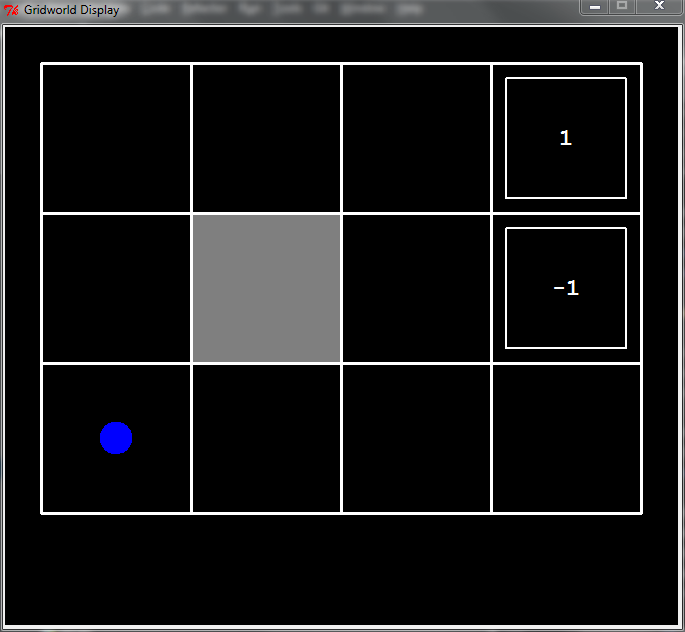
\includegraphics[scale=0.5]{image_1}
	\caption{Interfaz del dominio GridWorld en el modo de control manual.}
	\label{image_1}
\end{figure}

\subsection*{Preguntas}

\begin{questions}
	
% Pregunta 1
{ \question ¿Cuántas celdas/estados aparecen en el tablero? ¿Cuántas acciones puede ejecutar el agente? Si quisieras resolver el juego mediante aprendizaje por refuerzo, ¿cómo lo harías?\label{pregunta_1} 
}

En el tablero aparecen 11 celdas/estado y el agente puede ejecutar 4 acciones: arriba (\textit{north}), abajo (\textit{south}), izquierda (\textit{west}) y derecha (\textit{east}).

Para resolver el juego usaremos el algoritmo \href{https://en.wikipedia.org/wiki/Q-learning}{Q-learning} con el objetivo de que el agente llegue lo antes posible a la celda etiquetada con un 1 (estado \textit{done}), evitando caer en la celda con un -1 (estado \textit{exit}). La clave del algoritmo Q-learning será la construcción de su tabla \textit{Q}, que es una matriz donde tendremos las recompensas que obtendrá el agente para cada acción y en cada estado, es decir, los valores de $Q(s,a)$. El algoritmo hará que el agente vaya tomando decisiones y a cada decisión actualizará uno de los valores de $Q(s,a)$ de la tabla \textit{Q}. A la hora de tomar las decisiones el algoritmo usa la estrategia \textit{$\epsilon$}-greedy. Esta estrategia consiste en que todas las acciones sean tomadas buscando el valor máximo de $Q(s,a)$ pero existiendo una probabilidad pequeña, \textit{$\epsilon$}, de tomar una decisión aleatoria para que el agente explore todo el espacio de soluciones. Para la actualización de la tabla \textit{Q} e ir completándola, cada decisión tomada por el agente se evaluará por la siguiente expresión:

\begin{equation}
	\hat{Q}(s_{t}, a_{t}) \leftarrow (1-\alpha) \; \hat{Q}(s_{t}, a_{t}) + \alpha_{t} \; [r_{t+1} + \gamma \; max_{a} \; \hat{Q}(s_{t + 1}, a)]
\end{equation}

En esta expresión $\hat{Q}(s_{t}, a_{t})$ es el valor de la tabla \textit{Q} del estado $s_{t}$ y la acción $ a_{t}$. $\hat{Q}(s_{t}, a_{t})$ será el nuevo valor de la tabla \textit{Q} para dicho estado y acción. El valor $\gamma$ es el \href{https://en.wikipedia.org/wiki/Learning_rate}{\textit{learning rate}}, que puede tomar valores entre 0 y 1. Finalmente $r_{t+1}$, determina la recompensa inmediata asociada a la acción tomada y es el \href{https://en.wikipedia.org/wiki/Discounting#Discount_factor}{\textit{discount factor}} que también puede tomar valores entre 0 y 1.

% Pregunta 2
{ \question Abrir el fichero \textit{qlearningAgents.py} y buscar la clase \textit{QLearningAgent}. Describir los métodos que aparecen en ella.
}

Los métodos que aparecen en la clase \textit{QLearningAgent} son:

\begin{itemize}
	\item \textbf{\_\_init\_\_}: Inicializa la \textit{Q-Table} a partir del fichero \textit{qtable.txt}, es decir, la \textit{Q-Table} se inicializa a cero.
	
	\item \textbf{readQtable}: Lee la \textit{Q-Table} del fichero \textit{qtable.txt}.
	
	\item \textbf{writeQtable}: Escribe la \textit{Q-Table} en el fichero \textit{qtable.txt}.
	
	\item \textbf{\_\_del\_\_}: Llama al método \textit{writeQtable} que escribe el resultado final de la \textit{Q-Table} en el fichero \textit{qtable.txt}.
	
	\item \textbf{computePosition}: Calcula la fila de la \textit{Q-Table} para un estado dado.
	
	\item \textbf{getQValue}: Devuelve el valor $Q(s,a)$ para un estado y una acción dados. De lo contrario, devuelve 0.0, si nunca hemos visto el estado o el valor del nodo $Q$.
	
	\item \textbf{computeValueFromQValues}: Devuelve el valor máximo de $Q(s,a)$ para un estado dado. Este valor se encuentra por encima de las acciones válidas. Si no hay acciones válidas, como en el caso del estado \textit{exit}, devuelve 0.0.
	
	\item \textbf{computeActionFromQValues}: Calcula la mejor acción a realizar para un estado dado. Si no hay acciones válidas, como en el caso del estado \textit{exit}, devuelve \textit{None}.
	
	\item \textbf{getAction}: Calcula la acción a realizar para un estado dado. En caso contrario, con probabilidad \textit{self.epsilon}, elige una acción aleatoria y la mejor acción política. Si no hay acciones válidas, como en el caso del estado \textit{exit}, elige \textit{None} como acción.
	
	\item \textbf{update}: Actualiza la \textit{Q-Table}. El método para un acción dada, observa una recompensa, introduce un estado nuevo (que depende del estado anterior y de la acción dada), y actualiza el valor $Q(s,a)$. 
	
	Si el nuevo estado introducido es el estado \textit{exit}, se sigue la regla:
	
	\begin{center}
		$Q(state,action) <- (1-self.alpha) * Q(state,action) + self.alpha * (reward + 0)$
	\end{center}

	De lo contrario, si el nuevo estado introducido no es el estado \textit{exit}, se sigue la regla:
	
	\begin{center}
		$Q(state,action) <- (1-self.alpha) * Q(state,action) + self.alpha * (reward + self.discount * max a' Q(nextState, a'))$
	\end{center}
	
	\item \textbf{getPolicy}: Devuelve la mejor acción de la \textit{Q-Table} para un estado dado.
	
	\item \textbf{getValue}: Devuelve el valor $Q(s,a)$ más alto para un estado dado.
		
\end{itemize}

% Pregunta 3
{ \question Ejecuta ahora el agente anterior con: \textit{python gridworld.py -a q -k 100 -n 0}.}

A diferencia de la primera ejecución, en esta ejecución le indicamos el tipo de agente, que en este caso es q, y el número de movimientos/episodios \href{https://en.wikipedia.org/wiki/Markov_decision_process}{MDP} a realizar, que en este caso son 100.

\begin{figure}[h]
	\centering
	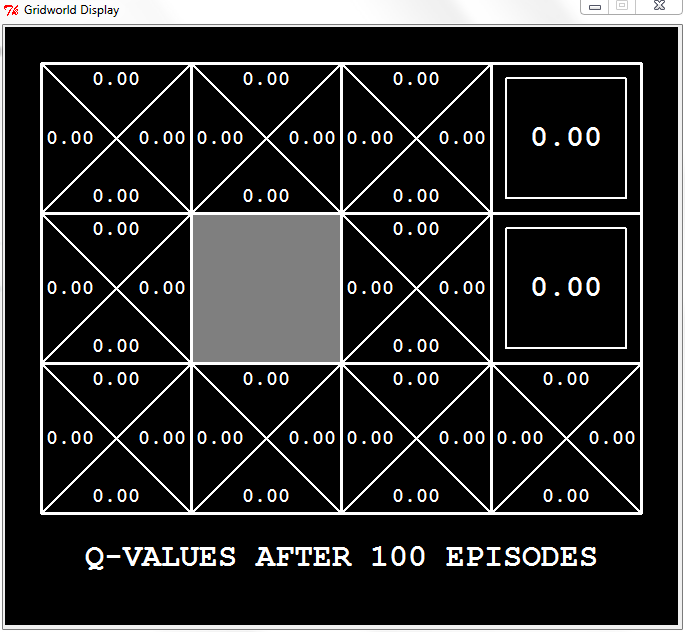
\includegraphics[scale=0.5]{image_2}
	\caption{Interfaz del dominio GridWorld usando \textit{python gridworld.py -a q -k 100 -n 0}.}
	\label{image_2}
\end{figure}

% Pregunta 4
{ \question ¿Qué información se muestra en el laberinto? ¿Qué aparece por terminal cuando se realizan los movimientos en el laberinto? 
}

Si observamos la Figura \ref{image_2}, vemos que la información que se muestra en el laberinto son los valores de $Q(s,a)$ después de realizarse 100 movimientos/episodios. Como la función de actualización (\textit{update}) de los valores de $Q(s,a)$ no se ha implementado aún, observamos que todos los valores de $Q(s,a)$ después de realizarse 100 movimientos son 0.

En la terminal cuando se realizan los movimientos/episodios, vemos que aparecen los siguientes valores por cada episodio hasta el estado TERMINAL\_STATE (\textit{exit}):

\begin{itemize}
	\item La posición (x, y) donde empieza el estado. Por ejemplo: (2, 1).
	\item La acción tomada. Por ejemplo: derecha (\textit{east}).
	\item La posición (x, y) donde acaba el estado. Por ejemplo: (3, 1).
	\item La recompensa obtenida. Por ejemplo: 0.0, en este caso no ha habido recompensa. 
\end{itemize}

Cuando se ha alcanzado en cada episodio el estado TERMINAL\_STATE, vemos que aparece por la terminal el valor máximo de $Q(s,a)$ de cada episodio. Por ejemplo: EPISODE 93 COMPLETE: RETURN WAS 0.0182480036314. Si hemos alcanzado el objetivo (la celda etiquetada con un 1) durante un episodio, tendremos una recompensa igual a 1 y el valor máximo de $Q(s,a)$ será positivo. Por el contrario, el valor máximo de $Q(s,a)$ será negativo y tendremos una recompensa igual a -1, al no alcanzar el objetivo y caer en la celda etiquetada con un -1. Así pues, consideramos que hemos ganado en un episodio si el valor máximo de $Q(s,a)$ del episodio es positivo, y consideramos que hemos perdido si el valor máximo de $Q(s,a)$ del episodio es negativo. En el caso del ejemplo, vemos que en el episodio 93 el valor máximo de $Q(s,a)$ es positivo, ganamos.

Finalmente, aparece en la terminal un último valor. Este valor es el promedio de todos los valores máximos de $Q(s,a)$ de todos los movimientos/episodios de una ejecución. Por ejemplo: AVERAGE RETURNS FROM START STATE: -0.079260284124. Con el planteamiento del párrafo anterior, si el promedio es negativo consideramos que hemos perdido la partida, y por el contrario si este valor es positivo consideramos que hemos ganado la partida. En el caso del ejemplo, vemos que el promedio es negativo, perdemos.

% Pregunta 5
{ \question ¿Qué clase de movimiento realiza el agente anterior?}

El agente desde una posición, siempre que decida moverse en una dirección por el laberinto, lo hace en esa dirección con probabilidad igual a 1, es decir, se mueve una posición. 

Este tipo de movimiento se define en un \href{https://en.wikipedia.org/wiki/Markov_decision_process}{proceso de decisión de Markov} (MDP, siglas en inglés) determinista, donde durante la ejecución de una acción desde un estado siempre se produce la misma transición de estado y la misma recompensa.

% Pregunta 6
{ \question ¿Se pueden sacar varias políticas óptimas? Describe todas las políticas óptimas para este problema.} 

En este caso, las políticas óptimas se inducen por la estimación de los valores máximos de $Q(s,a)$ y cambian después de cada movimiento/episodio. Los valores máximos de $Q(s,a)$ se almacenan en la tabla \textit{Q}. 

Así pues, se pueden sacar varias políticas óptimas si observamos la tabla \textit{Q}, que almacena todas la políticas óptimas para este problema. Concretamente observando la Tabla \ref{table_1}, o que es lo mismo, el fichero \textit{qtable.txt} que contiene la tabla \textit{Q} que almacena todas la políticas óptimas para este problema; vemos que tenemos 34 políticas óptimas donde parece que hemos alcanzado el objetivo (valores máximos de $Q(s,a) >$ 0).

\renewcommand{\tablename}{Tabla}

\begin{table}
	\centering
	\begin{tabular}{|c|c|c|c|c|}
		\hline
		0.590489969903 & 0.590489976465 & 0.531440972641 & 0.531440969095 & 0.0            \\ \hline
		0.590489859224 & 0.656099982789 & 0.590489980107 & 0.5314409716   & 0.0            \\ \hline
		0.728999990732 & 0.59048968547  & 0.656099948059 & 0.590489940173 & 0.0            \\ \hline
		0.0            & 0.590488144602 & 0.590489453559 & 0.656099880246 & 0.0            \\ \hline
		0.656099976912 & 0.59048996484  & 0.531440967592 & 0.590489963482 & 0.0            \\ \hline
		0.0            & 0.0            & 0.0            & 0.0            & 0.0            \\ \hline
		0.809999995782 & 0.0            & 0.656099462996 & 0.728999845279 & 0.0            \\ \hline
		0.0            & 0.0            & 0.0            & 0.0            & -1.0           \\ \hline
		0.65609997485  & 0.728999985783 & 0.590489975178 & 0.656099945627 & 0.0            \\ \hline
		0.728999987496 & 0.809999996062 & 0.728999945859 & 0.656099934053 & 0.0            \\ \hline
		0.809999962699 & 0.899999998166 & 0.728999985397 & 0.728999978711 & 0.0            \\ \hline
		0.0            & 0.0            & 0.0            & 0.0            & 0.999999999942 \\ \hline
	\end{tabular}
	\caption{Contenido del fichero \textit{qtable.txt} cuando \textit{epsilon} es igual a 1.}
	\label{table_1}
\end{table}

\newpage

% Pregunta 7
{ \question Escribir el método \textit{update} de la clase \textit{QLearningAgent} utilizando las funciones de actualización del algoritmo \textit{Q-Learning}. Para ello, inserta el código necesario allí donde aparezca la etiqueta INSERTA TU CÓDIGO AQUÍ siguiendo las instrucciones que se proporcionan, con el fin de conseguir el comportamiento deseado. }

El código que se ha insertado en el método \textit{update} de la clase \textit{QLearningAgent}, siguiendo las instrucciones que se proporcionan, es:

\begin{lstlisting}[language=Python]
position = self.computePosition(state)
action_column = self.actions[action]

if nextState != 'TERMINAL_STATE':
	# Q(state,action) <- (1-self.alpha) * Q(state,action) + self.alpha * (reward + self.discount * max a' Q(nextState, a'))
	sample = (1 - self.alpha) * self.getQValue(state, action) + self.alpha * (
		reward + self.discount * self.computeValueFromQValues(nextState))
	self.q_table[position][action_column] = sample

elif nextState == 'TERMINAL_STATE':
	# Q(state,action) <- (1-self.alpha) * Q(state,action) + self.alpha * (reward + 0)
	sample = (1 - self.alpha) * self.getQValue(state, action) + self.alpha * (reward + 0)
	self.q_table[position][action_column] = sample
\end{lstlisting}

En la Figura \ref{image_3} podemos observar que con el código insertado anteriormente, los valores de $Q(s,a)$ se han actualizado después de volver a ejecutar \textit{python gridworld.py -a q -k 100 -n 0}.

\begin{figure}[h]
	\centering
	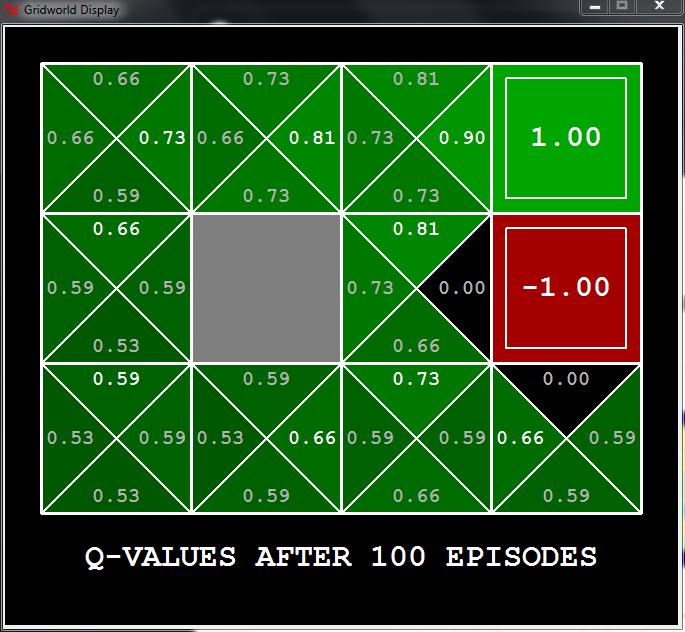
\includegraphics[scale=0.5]{image_3}
	\caption{Interfaz del dominio GridWorld cuando \textit{epsilon} es igual a 1.}
	\label{image_3}
\end{figure}

% Pregunta 8
{ \question Establece en el constructor de la clase \textit{QLearningAgent} el valor de la variable \textit{epsilon} a 0,05. Ejecuta nuevamente con: \textit{python gridworld.py -a q -k 100 -n 0}. ¿Qué sucede?
}

Cuando \textit{epsilon} es igual a 0,05:
\begin{itemize}
	\item AVERAGE RETURNS FROM START STATE: 0.530784257974.
\end{itemize}

Cuando \textit{epsilon} es igual a 1:
\begin{itemize}
	\item AVERAGE RETURNS FROM START STATE: -0.079260284124.
\end{itemize}

Cuando \textit{epsilon} es igual a 0,05, el promedio de todos los valores máximos de $Q(s,a)$ es positivo, por lo tanto, ganamos la partida después de todos los movimientos/episodios. Al contrario, cuando \textit{epsilon} es igual a 1, el promedio de todos los valores máximos de $Q(s,a)$ es negativo, por lo tanto, perdemos la partida después de todos los movimientos/episodios. Eso se debe a la estrategia $\epsilon$-greedy comentada anteriormente (ver Pregunta \ref{pregunta_1}), donde si el valor de $\epsilon$ es más pequeño, la probabilidad de que el agente tome decisiones aleatorias será menor. Si la aleatoriedad es menor, menor será la inestabilidad del algoritmo Q-learning.

\begin{figure}[h]
	\centering
	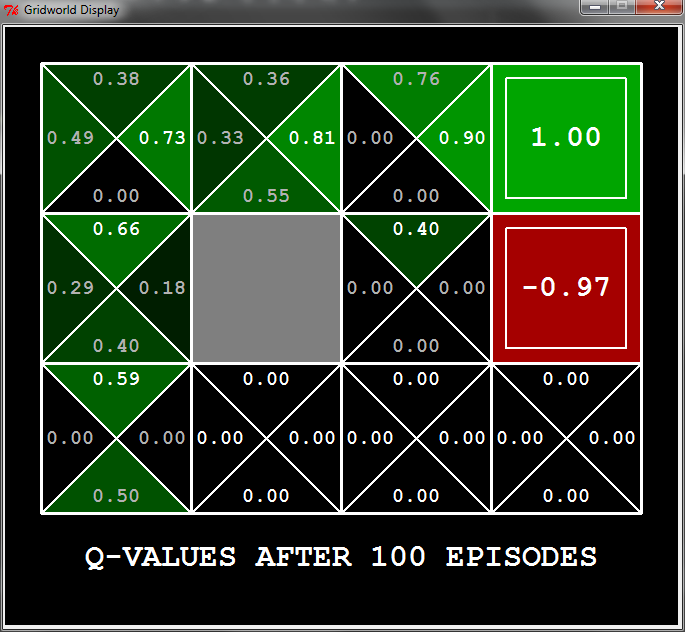
\includegraphics[scale=0.5]{image_4}
	\caption{Interfaz del dominio GridWorld cuando \textit{epsilon} es igual a 0,05.}
	\label{image_4}
\end{figure}

% Pregunta 9
{ \question Después de la ejecución anterior, abrir el fichero \textit{qtable.txt}. ¿Qué contiene?}

El fichero \textit{qtable.txt} contiene la tabla \textit{Q} que almacena los valores máximos de $Q(s,a)$, es decir, las políticas óptimas para este problema.

\begin{table}[h]
	\centering
	\begin{tabular}{|c|c|c|c|c|}
		\hline
		0.59049        & 0.119569809907 & 0.0            & 0.0            & 0.0   \\ \hline
		0.0            & 0.0            & 0.0            & 0.398575844342 & 0.0   \\ \hline
		0.0            & 0.0            & 0.0            & 0.0            & 0.0   \\ \hline
		0.0            & 0.0            & 0.0            & 0.0            & 0.0   \\ \hline
		0.6561         & 0.153677329102 & 0.0            & 0.4428675      & 0.0   \\ \hline
		0.0            & 0.0            & 0.0            & 0.0            & 0.0   \\ \hline
		0.568245849609 & 0.0            & 0.0            & 0.0            & 0.0   \\ \hline
		0.0            & 0.0            & 0.0            & 0.0            & -0.75 \\ \hline
		0.32805        & 0.729          & 0.295245       & 0.327896389246 & 0.0   \\ \hline
		0.0            & 0.81           & 0.364499433769 & 0.0            & 0.0   \\ \hline
		0.0            & 0.9            & 0.148078125    & 0.0            & 0.0   \\ \hline
		0.0            & 0.0            & 0.0            & 0.0            & 1.0   \\ \hline
	\end{tabular}
	\caption{Contenido del fichero \textit{qtable.txt} cuando \textit{epsilon} es igual a 0,05.}
	\label{table_2}
\end{table}

\end{questions}

\section*{Ejercicio 2}

En el ejercicio anterior, siempre que el agente decidía moverse hacia una dirección se movía en esa dirección con probabilidad 1. Es decir, se trataba de un MDP determinista. Ahora vamos a crear un MDP estocástico.

\subsection*{Preguntas}

\begin{questions}

% Pregunta 1
{ \question Ejecuta y juega un par de partidas con el agente manual: \textit{python gridworld.py -m -n 0.3}. ¿Qué sucede? ¿Crees que el agente \textit{QLearningAgent} será capaz de aprender en este nuevo escenario? \label{pregunta_1.2}.
}

Si ejecutamos \textit{python gridworld.py -m -n 0.3}, con el parámetro -n que añade ruido en la ejecución, sucede que a veces la dirección indicada no resulta la dirección deseada.

Creo que el agente \textit{QLearningAgent} será capaz de aprender en este nuevo escenario, aunque al haber añadido ruido se podría añadir el problema de la sobreestimación, que es la propiedad más dañina resultante del ruido. Sobretodo porqué en entornos ruidosos el algoritmo Q-learning a veces puede sobrestimar los valores de la acción, retrasando el aprendizaje.

% Pregunta 2
{ \question Reiniciar los valores de la tabla Q del fichero \textit{qtable.txt}.}

% Pregunta 3
{ \question Ejecutar el agente \textit{QLearningAgent}: \textit{python gridworld.py -a q -k 100 -n 0.3}.}

Con esta nueva ejecución obtenemos:

\begin{itemize}
	\item La Figura \ref{image_5}.
	\item La Tabla \ref{table_3}, que contiene la tabla \textit{Q} del fichero \textit{qtable.txt}.
\end{itemize}

\renewcommand{\tablename}{Tabla}

\begin{table}[h]
	\centering
	\begin{tabular}{|c|c|c|c|c|}
		\hline
		0.553445100458 & 0.105618413429 & 0.199229717446 & 0.24706559221   & 0.0             \\ \hline
		0.340125559311 & 0.20729569976  & 0.142353922    & 0.0             & 0.0             \\ \hline
		0.492279805329 & 0.0            & 0.0            & 0.0             & 0.0             \\ \hline
		0.0            & 0.0            & 0.0            & 0.0             & 0.0             \\ \hline
		0.598455517406 & 0.349085290292 & 0.373117962712 & 0.352953780041  & 0.0             \\ \hline
		0.0            & 0.0            & 0.0            & 0.0             & 0.0             \\ \hline
		0.311843501505 & 0.0            & 0.0            & 0.0794004649324 & 0.0             \\ \hline
		0.0            & 0.0            & 0.0            & 0.0             & -0.999755859375 \\ \hline
		0.536520688909 & 0.699846713972 & 0.284330620577 & 0.0             & 0.0             \\ \hline
		0.222647958984 & 0.788829333025 & 0.0            & 0.505855779933  & 0.0             \\ \hline
		0.730856716955 & 0.894327291772 & 0.486130902902 & 0.520064147566  & 0.0             \\ \hline
		0.0            & 0.0            & 0.0            & 0.0             & 1.0             \\ \hline
	\end{tabular}
	\caption{Contenido del fichero \textit{qtable.txt} cuando \textit{epsilon} es igual a 0,05 y existe ruido.}
	\label{table_3}
\end{table}

\newpage

% Pregunta 4
{ \question Tras unas cuantos episodios, ¿se genera la política óptima? Y si se genera, ¿se tarda más o menos que en el caso determinista?
}

Tras unos cuantos episodios se genera la política óptima y cuando se genera tarda más que en el caso determinista. Si en el caso determinista, la mejor política óptima se encontraba en el movimiento/episodio 8, en el caso estocástico se encuentra en el episodio 22. Se tarda bastante más, seguramente por el problema de sobreestimación comentado anteriormente en la Pegunta \ref{pregunta_1.2}.

\begin{figure}[h]
	\centering
	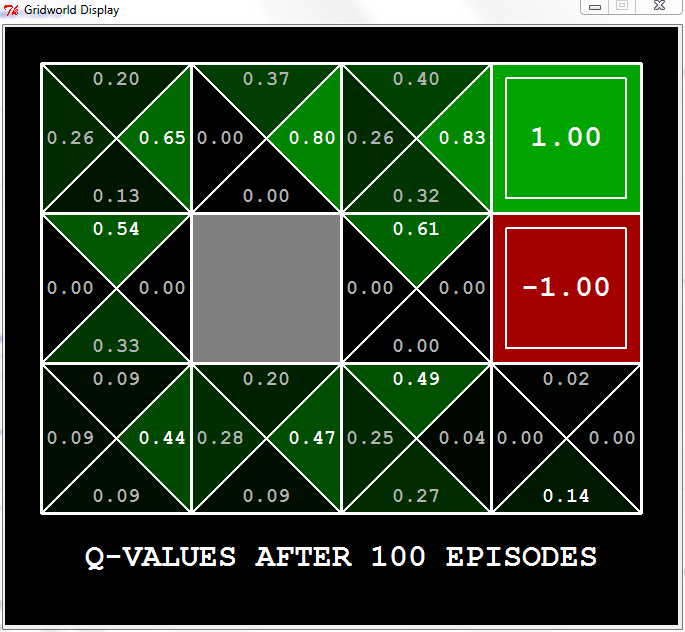
\includegraphics[scale=0.5]{image_5}
	\caption{Interfaz del dominio GridWorld cuando \textit{epsilon} es igual a 0,05 y existe ruido.}
	\label{image_5}
\end{figure}

\end{questions}

Todo el contenido de esta práctica se puede encontrar en el repositorio personal de GitHub: \url{https://github.com/lrodrin/masterAI/tree/master/A21/softpractica1}.

\end{document}
